\documentclass[a4paper,10pt]{article}
\usepackage[utf8]{inputenc}
\usepackage{float}
\usepackage{pgfplotstable}
\usepackage{amsfonts}
\usepackage{listings}
\usepackage[parfill]{parskip}

% \float­place­ment{fig­ure}{H}
\pgfplotsset{compat=1.13}

\pgfplotstableread[col sep=comma]{
Dataset,MAP,NB,TANB
Mushroom,0.51,0.95,0.99
Votes,0.52,0.9,0.93
Pima,0.35,0.63,0.53
Titanic,0.79,0.77,0.79
CM, 0.23,0.51,0.5
German,0.3,0.71,0.65
}\mytable

\pgfplotstableread[col sep=comma]{
Dataset,MAP,NB,TANB
Mushroom,1,0.95,1
Votes,1,0.9,0.95
Pima,1,0.86,0.95
Titanic,0.79,0.78,0.79
CM, 0.95,0.54,0.73
Lenses,1,0.96,0.86
Weather,1,0.85,0.92
German,1,0.84,1
}\degenerate

\pgfplotstableread[col sep=comma]{
Dataset,MAP,NB,TANB
Mushroom,0.5,0.95,1
Votes,0.56,0.86,0.87
Pima,0.51,0.73,0.48
Titanic,0.69,0.70,0.69
CM, 0.32,0.45,0.51
German,0.5,0.76,0.48
}\sensitivity

\pgfplotstableread[col sep=comma]{
Dataset,MAP,NB,TANB
Mushroom,0,0.96,1
Votes,0.66,0.86,0.88
Pima,0.65,0.73,0.48
Titanic,0.80,0.76,0.82
CM, 0.32,0.46,0.51
German,0,0.74,0.44
}\precision


\definecolor{blueaccent}{RGB}{0,150,214}
\definecolor{greenaccent}{RGB}{0,139,43}
\definecolor{purpleaccent}{RGB}{130,41,128}
\definecolor{orangeaccent}{RGB}{240,83,50}


%opening
\title{Bayesian classifiers in action with Scala}
\author{Pol Alvarez Vecino}

\begin{document}

\maketitle

\begin{abstract}

This project explores some basic probability-based classifiers, addresses some of the issues they present, and finally uses cross-validation to compare them against a batch of datasets. 

\end{abstract}

\section{Introduction}

The project's goal is to implement three basic classifiers, Maximum a Posteriori, Naive Bayes, and Tree-Augmented Naive Bayes, and compare their performance. The implementation is done in Scala \cite{Odersky2011}, a general purpose language with OO, functional programming, and strong static typing which runs in the JVM and is designed to overcome many of Java problems and critics. Scala was chosen because it is oriented towards functional programming which allows easier parallelizations which could be very useful for ML-related tasks.

To test the implementations performance we created an orchestrating main class called \textit{PredictorsTest.scala}. The class runs the three different algorithms for each dataset twice: first with 10x10CV (see Subsection \ref{subsec:validation}, and a second time with the whole dataset as train and test (see Section \ref{sec:experiments}). It is also responsible of creating and updating the Confusion Matrix. To keep the code simple, this class defines a trait\footnote{traits are scala's equivalent of interfaces} called \textbf{classifier} that all classifiers must implement. It defines a getter function for the class variable values (required to build the confusion matrix) and the predict method which takes a sample as argument and returns a list of predictions. This trait is implemented by the three methods making their testing equal regardless the classifier.

The code is well structured and heavily commented so this document will only mention the more theoretical details of the implementation inviting the reader to check the actual code.

\section{Max a Posteriori}

Associated files:
\begin{description}
 \item [· MaxAPosteriori.scala,] contains class implementing Maximum a Posteriori classifier
\end{description}


Maximum a Posteriori (MAP) is quite straight forward and can be easily understood checking the actual code. It is worth mentioning that for convenience during tests and comparisons, the conditional probabilities data structure has a default value of 0. This means that when encountering a key not seen during training, instead of crashing, the algorithm attributes 0 probability to the prediction. The variability introduced by this random predictions is very high when using 10x10CV heavy limiting its accuracy, nonetheless the results are added for reference.


\section{Naive Bayes}

Associated files:
\begin{description}
 \item [· NaiveBayes.scala,] contains class implementing Naive Bayes classifier
\end{description}

  Naive Bayes classifier implementation structure follows the one provided in the lab. The probability formula is given by:
  \begin{equation}
  P(x) = P(\omega_k) * \prod_{j=1}^d P(X_j=x_j|\omega_k)
  \end{equation}

Naive Bayes predictor (NB) implements the basic classifier and counting methods to create the conditional probabilites but is improved with some more features. The null values are again treated with the 0 default value. However, having a null probability for an attribute turns the whole prediction to 0. To avoid that we use Laplace correction as described in subsection \ref{subsec:laplace}.

Using Scala functional programming features, the prediction method is parametrized with 3 functions: probability formula, probability filter, and accumulate function. The \textbf{probability function} specifies how to compute the probability given the numerator and denominator of the fraction, thanks to this it is possible to use simple probability or Laplace correction (described in next section). The \textbf{probability filter} and \textbf{accumulate function} are used to implement the simple or log probability, the filter is either $f(x) = x$ or $f(x) = log(x)$, the accumulation just describes if the probabilities shoud be summed of multiplied.

This combinations result in 4 execution modes:

\begin{enumerate}
  \item Simple probability without Laplace correction
  \item Log probability without Laplace correction
  \item Simple probability with Laplace correction
  \item Log probability with Laplace correction
\end{enumerate}


\subsection{Log probability}

In order to avoid numerical precision problems when multiplying really small probabilities, the log probability formula \ref{eq:log} is used to predict new values. Logarithms are a strictly increasing function so we can use them to turn the product into a sum avoiding numerical issues while retaining the same prediction ordering. It is worth noting that when applying logs the results are no longer probabilities (can be bigger than 1).

\begin{equation} \label{eq:log}
 P(x) = ln P(\omega_k) * \sum_{j=1}^d ln P(X_j=x_j|\omega_k)
\end{equation}


\subsection{Laplace correction}
\label{subsec:laplace}
Laplace correction formula \ref{eq:laplace} prevents null probabilites (i.e. a 0 value in a conditional probability) from turning the final prediction into 0, for simple probabilities, or tend to infinity when using log probabilites. Roughly speaking, the correction applies a constant term to both numerator a denominator to prevent the 0 value. This value is the prior probability of each class (assuming they are all equal) which is defined by $1/V_k$ being $V_k$ the number of classes. This prior probability is weighted with a factor $p$ whose value should be optimized (for example with cross validation). In this paper, when using Laplace correction, the value of $p$ is always 1.

\begin{equation} \label{eq:laplace}
 P_L(X_j = x_j | \omega_k ) = \frac{ | \{ x \in S_k \land X_j = x_j \} | + p }{ | \{ x \in S_k \} | + p*V_k}, p \in \mathbb {N} 
\end{equation}



\section{Tree-Augmented Naive Bayes}
Associated files:
\begin{description}
 \item [· TANaiveBayes.scala,] contains class implementing Tree-Augmented Naive Bayes classifier
 \item [· UnionFindSet.scala,] union-find set data structure for Kruskal algorithm \cite{Kruskal1956}
 \item [· TANTree.scala,] contains class TANTree which holds all information required for prediction
\end{description}

Tree Augmented Naive Bayes \cite{Uther2011} (TANaiveBayes or TANB) method tries to soften the independence assumption between variables of Naive Bayes with a tree-like dependency structure. In the structure, each variable represents a node of the tree and its conditional probability depends on the class variable and its parent node. The probability is given by the formula in equation \ref{eq:tanb}.

\begin{equation} \label{eq:tanb}
 P(x) = P(\omega_k) * P(X_{root}|\omega_k) * \prod_{j=2}^d  P(X_j=x_j|\omega_k, X_{j.parent})
\end{equation}

Worth noting is that the root of the tree just depends on the class variable so it is out of the product (index starts at 2). As in Naive Bayes, the prediction was parametrized to be able to use log-probabilites and Laplace correction. 

The tree is built in five steps:

\begin{enumerate}
 \item Compute conditional mutual information for each different pair of attributes.
 \item Build a graph with each attribute as a node and each edge annotated with their mutual information.
 \item Build a maximum weighted spanning tree.
 \item Turn the undirected tree to directed one by choosing a variable and setting all to flow out of it.
 \item Link all nodes to a new node representing class variable.
\end{enumerate}

Detailed information of the process in \cite{Uther2011} and \cite{Padmanaban2014}. This implementation was more complex than previous classifiers so it was split into three classes.

The main class, TANaiveBayes, is responsible of implementing the classifier trait, and performing steps 1-3. Once the maximum weighted tree is built, it is fed to the TANTree class which directs the tree and stores all the information required to make a prediction. With this setup, TANaiveBayes acts as a constructor and wrapper for the TANTree class because it computes the required info for the tree and its method predict calls TANTree.predict. Figure \ref{fig:tantree} shows the dependencies tree generated for Votes classifier. Inspecting the actual dependencies is out of scope, but one quick look shows a meaningful relation: politicians voting to spend on el Salvador aid also voted for aid to Nicaragua (more details about the datasets in Subsection \ref{subsec:datasets}).

\begin{figure}[H]
\centering
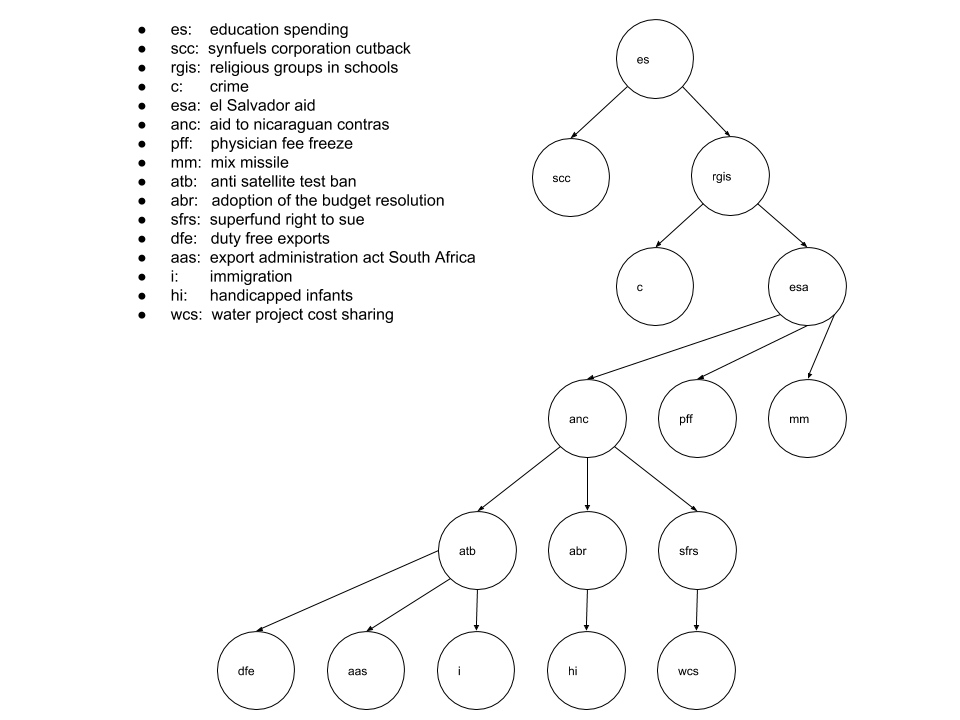
\includegraphics[keepaspectratio, width=9cm]{images/TANTree.png}
\caption{Tree structure of TANaiveBayes classifier for dataset \textit{votesTr.txt}. The goal is to predict if a politician is republican or democrat based on his budget spending votes.}
\label{fig:tantree}
\end{figure}

\section{Experiments}
\label{sec:experiments}

Associated files:
\begin{description}
 \item [· PredictorsTest.scala,] file orchestrating all the tests execution.
 \item [· ConfusionMatrix.scala,] class containing the confusion matrix and diverse test metrics.
\end{description}

In order to reproduce the experiments performed Scala 2.11 is required. To compile and execute the tests issue the Listing 1. commands inside the folder \textit{"./classifiers/src"}.

\begin{lstlisting}[language=bash,caption={Compilation and execution commands to reproduce reported results}]
scalac -cp . *.scala
scala -cp . TestsExecutor
\end{lstlisting}

Note that even if the main file is PredictorsTest when executing the code we must use the object inside the file name: TestExecutor.
As explained previously two kind of tests have been performed for each method. First method with 10x10CV, second with whole dataset as train and test. 

\subsection{Datasets}
\label{subsec:datasets}

List of the datasets used and their classification objective:

\begin{description}
 \item [· cmcTr.txt,] contraceptive method used.
 \item [· lensesTr.txt,] kind of lenses to wear (or none).
 \item [· WeatherNominalTr.txt,] play tenis depending on the weather.
 \item [· mushroomTr.txt,] predict if a Mushroom is edible or toxic.
 \item [· votesTr.txt,] democrat or republican politican.
 \item [· pimaTr.txt,] predict if an individual has diabetes \cite{Smith}
 \item [· titanicTr.txt,] surival to the Titanic accident.
 \item [· germanTr.txt,] german language level.
\end{description}

All the datasets are formated following libsvm format with the exception that class value is the last one (instead of the first) and is named (classLabel:classValue). Lenses and WeatherNominal are small test datasets so they are not used when computing validation error with 10x10CV because too few samples per fold would be available and results would be highly biased (specially with MAP classifier which chooses randomly when the posterior probability for an attribute is null). Despite that, we have also executed all the datasets without validation (whole dataset for train and test) for reference and comparison.


\subsection{Cross-validation}
\label{subsec:validation}

The validation method used in the experiments is 10-fold and 10 iterations cross-validation (10x10CV). For each method and dataset, data is shuffled and 10 cross-validation is performed. This is repeated 10 times, reshuffling data every time. The final model accuracy is the average of all partial ones.

As stated \textit{Lenses} and \textit{WeatherNominal} datasets were not used during 10CV because they were too small.

\subsection{Contingency matrix for muticlass problems}

Contingency matrix implementation was first translated from the python implementation seen in the labs. Afterwards, we added the accuracy, precision, specificity, and sensitivity metrics to it. However, the inclusion of the \textit{Lenses} and \textit{Contraceptive Method} datasets, which are multi-class problems, required to revise the contingency matrix implementation and reported measures. 

The matrix extension to an arbitrary number of classes was trivial, reporting in a list all the possible combinations of predicted-truth labels. For the metrics, the sensitivity and precision become a per-class metric (measuring the true-positives against all the other classes). Mean sensitivity and precision of all the classes is also reported. Specificity metric is no longer used because it is computed the same way as the sensitivity (having 2+ classes means there are no longer negative labels, they are just the positive labels of one of the rest targets).

\section{Results}
\label{subsec:contingency}

Figure \ref{fig:degenerate} shows the accuracy results of each classifier and dataset when using all the data as training and validation. Maximum a Posteriori has, as expected, perfect accuracy in all consistent datasets (same attributes imply same class) because it simply memorizes all combinations. The decrease in accuracy observed in NB is caused by the independence assumption between the variables. This same reason is the one causing TANaiveBayes to have improved accuracy over NB because it can represent and take into account some of the dependencies between the variables.

\begin{figure}[H]
\begin{tikzpicture}
  \begin{axis}[
    width=1*\linewidth,
    height=250pt,
    ybar,
    bar width=7.5pt,
    ymin=0.5,
    enlarge x limits={abs=25pt},
    legend style={draw=none,at={(0.5,-0.15)},
    anchor=north,legend columns=-1},
    xlabel={Datasets},
    ylabel={Accuracy},
    symbolic x coords={Mushroom, Votes, Pima, Titanic, CM, Lenses, Weather, German},
    xtick=data,
    cycle list={blueaccent,greenaccent,purpleaccent}
  ]
    \pgfplotsinvokeforeach{MAP,NB,TANB}{
      \addplot+[draw=none,fill,] table[x=Dataset,y=#1]{\degenerate};
      \addlegendentry{#1}
    }
\end{axis}
\end{tikzpicture}
\caption{Accuracy for each classifier and dataset using the whole dataset for training and validation. MAP accuracy is 1.0 for all datasets which do not contain contradictory samples (same attributes different class). TANaiveBayes outperforms NB in almost all datasets. The performance increase is most probably related to the actual independence of the variables (NB assumption) and the tree ability to represent the dependencies.}
\label{fig:degenerate}
\end{figure}

Figure \ref{fig:accuracy} shows the mean accuracy of the ten iterations with 10CV.

The big decrease in MAP accuracy, sensitivity, and precision is due to the increased null probabilites when leaving out observations that cause biased predictions (predicts always first class).

\begin{figure}[H]
\begin{tikzpicture}
  \begin{axis}[
    width=0.8*\linewidth,
    ybar,
    bar width=7.5pt,
    ymin=0,
    enlarge x limits={abs=25pt},
    legend style={draw=none,at={(0.5,-0.15)},
    anchor=north,legend columns=-1},
    xlabel={Datasets},
    ylabel={Sensitivity},
    symbolic x coords={Mushroom, Votes, Pima, Titanic, CM, German},
    xtick=data,
    cycle list={blueaccent,greenaccent,purpleaccent}
  ]
    \pgfplotsinvokeforeach{MAP,NB,TANB}{
      \addplot+[draw=none,fill,] table[x=Dataset,y=#1]{\mytable};
      \addlegendentry{#1}
    }
\end{axis}
\end{tikzpicture}
\caption{Accuracy for each classifier and dataset using 10x10CV}
\label{fig:accuracy}
\end{figure}

NB and TANB accuracies are now much closer and we do not see a consistent improvement when using the later. This could be because when using 10x10CV the TANB has more difficulties to learn the correct dependencies among variables. Another option is that, for some folds or iterations, the shuffling produces a model with an awful accuracy making the mean decrease notably. Finally, it could also indicate that for some datasets the variables are actually independent (or close) and trying to figure out dependencies between them is useless and just add noise. 

Figure \ref{fig:sensitivity}, and \ref{fig:precision} show the mean sensitivity and precision of the first fold of the first iteration of 10CV for reference (actual values may vary a lot but it provides some insight). It is interesting to see that for German dataset TANaiveBayes classifier is far less sensible and precise than NB but its accuracy remains close enough. This can be caused by imbalance in the class of the samples because for a class the sensitivity may be really bad and for the other acceptable. This will lead to a bad mean. Despite that, if the class with better sensitivity occurs much more frequently the overall accuracy will be good enough. The same argument can be applied to precision, leading to the obseved acceptable accuracy with an awful precision and sensitivity. Again is worth noting that precision and sensitivities come from a single iteration and the reasoning could be biased.


\begin{figure}[H]
\begin{tikzpicture}
  \begin{axis}[
    width=0.8*\linewidth,
    ybar,
    bar width=7.5pt,
    ymin=0,
    enlarge x limits={abs=25pt},
    legend style={draw=none,at={(0.5,-0.15)},
    anchor=north,legend columns=-1},
    xlabel={Datasets},
    ylabel={Sensitivity},
    symbolic x coords={Mushroom, Votes, Pima, Titanic, CM, German},
    xtick=data,
    cycle list={blueaccent,greenaccent,purpleaccent}
  ]
    \pgfplotsinvokeforeach{MAP,NB,TANB}{
      \addplot+[draw=none,fill,] table[x=Dataset,y=#1]{\sensitivity};
      \addlegendentry{#1}
    }
\end{axis}
\end{tikzpicture}
\caption{Sensitivity for each classifier and dataset using 10x10CV}
\label{fig:sensitivity}
\end{figure}


\begin{figure}[H]
\begin{tikzpicture}
  \begin{axis}[
    width=0.8*\linewidth,
    ybar,
    bar width=7.5pt,
    ymin=0,
    enlarge x limits={abs=25pt},
    legend style={draw=none,at={(0.5,-0.15)},
    anchor=north,legend columns=-1},
    xlabel={Datasets},
    ylabel={Precision},
    symbolic x coords={Mushroom, Votes, Pima, Titanic, CM, German},
    xtick=data,
    cycle list={blueaccent,greenaccent,purpleaccent}
  ]
    \pgfplotsinvokeforeach{MAP,NB,TANB}{
      \addplot+[draw=none,fill,] table[x=Dataset,y=#1]{\precision};
      \addlegendentry{#1}
    }
\end{axis}
\end{tikzpicture}
\caption{Precision for each classifier and dataset using 10x10CV}
\label{fig:precision}
\end{figure}

\section{Conclusions and Future Work}

The resulting implementation in Scala is quite clean (for being first time programming with it) and understandable despite being a bit bloated with long parameter types. The static typing system helped to avoid some problems that arise easily in python and also makes the code more legible when dealing with complex data structures such as the TANTree. The probability computation and conditional mutual information loops, which are the most computation-intensive parts, are separated methods which makes them easy to parallelize. 

With respect to TANaiveBayes, the method had good results although not significative enough (could be the reason why they are not one of the most applied methods). As future work we could try to manually construct the dependencies tree (or at least tweak it) with the help of an expert of the data and see if that yields better results. 

Finally, we have extended the confusion matrix, accuracy, and sensitivity for muticlass problems and decided how to average and report them when dealing with 10x10CV. Despite that, we have seen that the gathered results, even if useful, did not provide enough information to clear picture of the performance. It would be interesting to complement these numerical results with ROC curves and more detailed metrics (were averaging does not hide or bias the regular values). 

\bibliography{bibliography} 
\bibliographystyle{ieeetr}

\end{document}
